\FloatBarrier
\subsection{Changed opponents and work calibration}
\label{app:public-stock-robustness}
The next fixed study retains both finalists and control. Each actor now faces
the other retained parent's adapted policy under the same rule. Rollouts and
continuation tables still use the actor's own fixed policy: the search receives
neither an opponent oracle nor hidden opponent cards. The six policy/table
systems are reused without new training or table preparation in this study.

Thirty-two separate duplicate streams, both seats, calibrate work at 32 worlds
per action. These 384 pilot matches use 55,378,349 planning transitions.
Only observed work sets the later particle counts: round target divided by
transitions per match per particle to the nearest integer, with half-up ties
and a $[2,256]$ clamp. Targets are 60,000 and 240,000 transitions per match.
The resulting low/high counts are 24/95 and 23/94 for control, 10/40 and
10/38 for preview plus choice, and 12/49 and 13/50 for all three.
These target expected work, not a hard per-match cap or equal wall time.

Evaluation uses 128 new duplicate streams shared by all arms, both seats,
the three rules, two parents and zero/low/high budgets: 4,608 actual matches,
32,587 rounds and 725,475 scored decisions. All decisions are replayed in
Python; independent reduction reproduces outcomes and evaluation counts.
Recorded search work is 32,934,469 rollouts and 449,378,614 transitions across
235,771 roots. These internal rollout counters are not independently replayed.
The round-completion search and its 2.5-standard-error guard remain unchanged.

Fourteen prespecified comparisons use 20,000 paired-stream bootstrap
replicates and two-sided Bonferroni quantiles $0.05/28$ and $1-0.05/28$.
The nominal 95\% familywise target applies within this study only. For each
finalist, gain over zero, excess over control and high-minus-low gain must
have positive lower bounds for both parents. A finalist ranking requires
both paired difference intervals to exclude zero in the same direction.

\begin{table}[ht]
\centering\small
\begin{tabular}{lllrrr}
\toprule
Rule & Parent & Comparison & Mean & Lower & Upper \\
\midrule
Preview + choice & 0 & High--zero & +25.39 & +16.21 & +34.96 \\
Preview + choice & 0 & Excess over control & +23.63 & +12.89 & +33.98 \\
Preview + choice & 0 & High--low & +14.65 & +5.27 & +24.22 \\
Preview + choice & 1 & High--zero & +19.92 & +11.52 & +28.77 \\
Preview + choice & 1 & Excess over control & +18.16 & +7.62 & +28.52 \\
Preview + choice & 1 & High--low & +2.73 & -6.05 & +11.52 \\
All three & 0 & High--zero & +26.95 & +17.97 & +36.33 \\
All three & 0 & Excess over control & +25.20 & +15.23 & +35.16 \\
All three & 0 & High--low & +14.84 & +6.25 & +23.83 \\
All three & 1 & High--zero & +28.71 & +19.34 & +38.28 \\
All three & 1 & Excess over control & +26.95 & +16.02 & +37.89 \\
All three & 1 & High--low & +13.67 & +5.02 & +22.46 \\
Preview + choice minus all three & 0 & Gain difference & -1.56 & -14.06 & +10.41 \\
Preview + choice minus all three & 1 & Gain difference & -8.79 & -20.12 & +2.99 \\
\bottomrule
\end{tabular}

\caption{All fourteen changed-opponent comparisons, in percentage points.
Intervals are simultaneous paired-bootstrap intervals under the fixed V4
family. Excess subtracts the corresponding control's high-minus-zero gain.
The last two rows compare the finalists' gains, not absolute strength across
different games. Scores count ties as one half.}
\label{tab:public-stock-robustness-comparisons}
\end{table}

All three passes all six score inequalities. Its high-budget gains are
26.95/28.71 points, and increasing low to high adds 14.84/13.67 points,
with simultaneous lower bounds 6.25/5.02. Preview plus choice also has positive
gain and excess bounds for both parents, but its parent-1 high-minus-low
change is 2.73 points with interval $[-6.05,11.52]$; its six-inequality
criterion therefore fails. Neither finalist-difference interval excludes
zero, so their ranking remains unresolved.

\begin{figure}[ht]
\centering
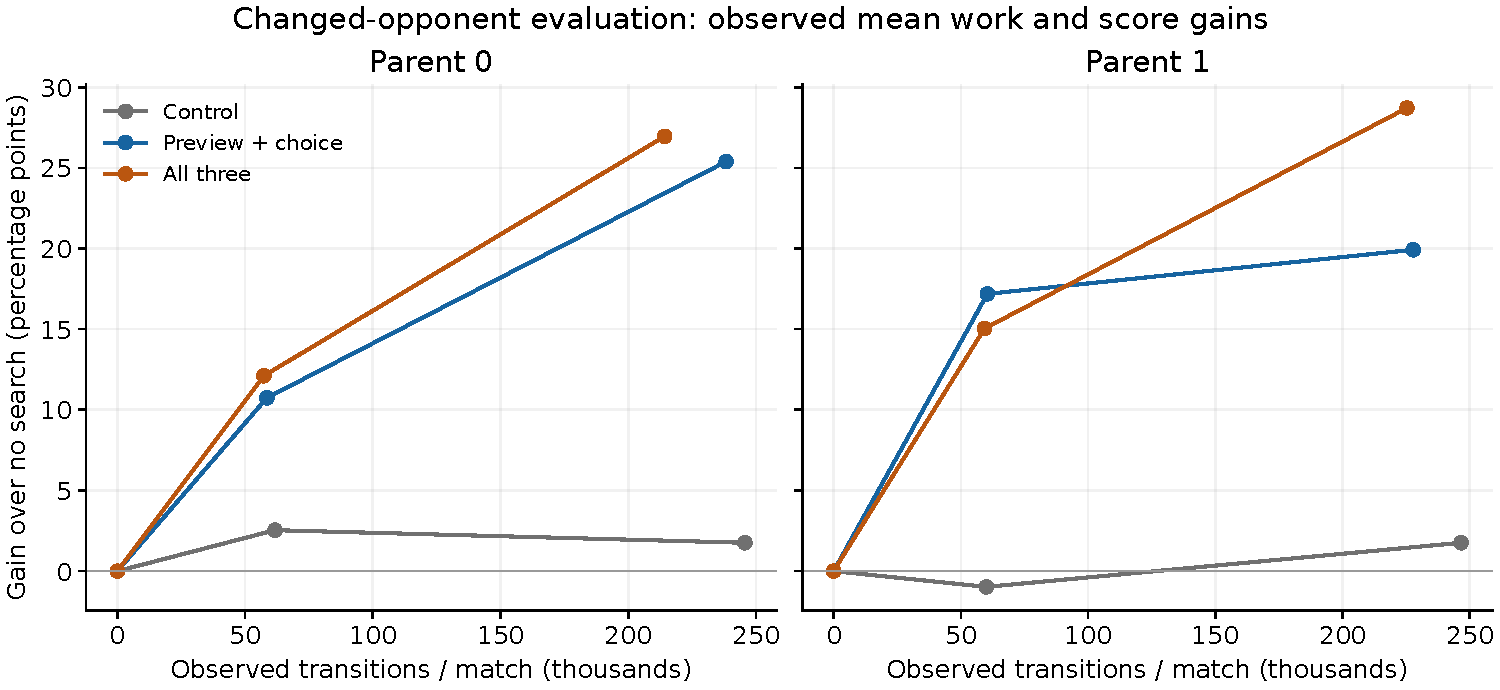
\includegraphics[width=\linewidth]{generated/public_stock_v4/public_stock_robustness_work.pdf}
\caption{Changed-opponent mean gains against observed online work. Each
curve starts at its own no-search score. Points show the three fixed budgets;
connecting lines do not assert a response between tested budgets.
Simultaneous comparisons are in Table~\ref{tab:public-stock-robustness-comparisons}.
Inference, preparation and wall time are not included in transition counts.}
\label{fig:public-stock-robustness-work}
\end{figure}

\begin{table}[ht]
\centering\small
\begin{tabular}{llrrrrl}
\toprule
Rule & Parent & Target (k) & Worlds & Actual (k) & Error (\%) & Pass \\
\midrule
Control & 0 & 60 & 24 & 61.72 & +2.86 & Yes \\
Control & 0 & 240 & 95 & 245.67 & +2.36 & Yes \\
Control & 1 & 60 & 23 & 60.01 & +0.02 & Yes \\
Control & 1 & 240 & 94 & 246.62 & +2.76 & Yes \\
Preview + choice & 0 & 60 & 10 & 58.52 & -2.46 & Yes \\
Preview + choice & 0 & 240 & 40 & 238.33 & -0.70 & Yes \\
Preview + choice & 1 & 60 & 10 & 60.43 & +0.72 & Yes \\
Preview + choice & 1 & 240 & 38 & 227.78 & -5.09 & Yes \\
All three & 0 & 60 & 12 & 57.36 & -4.41 & Yes \\
All three & 0 & 240 & 49 & 214.28 & -10.72 & No \\
All three & 1 & 60 & 13 & 59.30 & -1.16 & Yes \\
All three & 1 & 240 & 50 & 225.35 & -6.11 & Yes \\
\bottomrule
\end{tabular}

\caption{All twelve held-out work checks. Target and actual work are
thousands of physical rollout transitions per match; worlds are per legal
root action. Every endpoint must be within 10\% of its target for the
registered matched-work claim.}
\label{tab:public-stock-robustness-costs}
\end{table}

Eleven of twelve work checks pass. The all-three parent-0 high arm uses
214,281.81 transitions per match, 10.72\% below its 240,000 target.
The full matched-work criterion thus fails, and no matched-work ranking is
established. We retain the changed-opponent score evidence and every observed
cost; we do not retune or extend the cohort. The all-three result demonstrates
additional-computation value under a changed fixed opponent, while calibrated
work equality and stronger-policy robustness remain separate questions.
The conditional adaptation study must first measure improvement against both
retained opponents before a new-policy search replication.
\FloatBarrier
